%!TEX root = ../dissertation.tex
\begin{savequote} 75mm 
The Secret of Happiness lies in looking at all the wonders of the world and never forgetting the two drops of oil in the spoon.
\qauthor{The alchemist, Paulo Coelho}
\end{savequote}

\chapter{Materials and methods}

\section{Shell fabrication}
\subsection{Motivations}
\paragraph{}
This study requires a full control over the geometry, the material and the manufacturing process to ensure the reproducibility of the experiments.\\
Further more, two constraints were to take into account: the ability to induce the buckling within a pressure range of -1 bar and 1 bar and the ability to apply several cycles without damaging the shell. 
\paragraph{}This implies that the material to be used needs to have a high tensile strength to withstand the deformation cycle without entering the plastic domain and a rigidity small enough to trigger a buckling in the imposed pressure range and a feasible $(\frac{d}{R})$ range i.e $d > 1 mm$ and $R < 50 mm$. Visco-elastic polymers called elastomers qualify to these prerequisites and have been chosen for the shell manufacturing.
\paragraph{}
Before deciding to manufacture spherical hollow shells, we tried different kind of commercial "`balls"'. It was not conclusive because the process of fabrication was not intended to be reproducible in terms of material composition, thickness or diameter. This is why it was decided to manufacture them.
\paragraph{}
Several techniques were considered to manufacture polymer-based spherical hollow shells, including 3D-printing, rotational molding, processes involving high-pressure vulcanization. These techniques would have required either buying expensive equipments or subcontracting to a company with inconveniences of time delay, loss of control over the process and expensive cost of prototyping. 
The most suitable solution was the more common bi-molding process where the two halves of an object are cast and then assembled. The main advantages being the cost and the low-time consumption, plus a total control over the process, which includes the choice of materials, the reproducibility and more freedom over the geometry.
\subsection{Molding equipments}

\paragraph{\textbf{Female mold:}}
It consists of a cylinder of radius $R_{cylinder}=30 mm$  hollowed out to produce a half a sphere imprint of radius $R_{out}=25 mm$ and a height of $h = 30 mm$ (see fig.\ref{fig:female_mold}). The concavity is where the casting material is poured.
A groove was added to store any potential material surplus. Two female molds are necessary for the casting operation.
\begin{figure}[h] %
	\centering%
		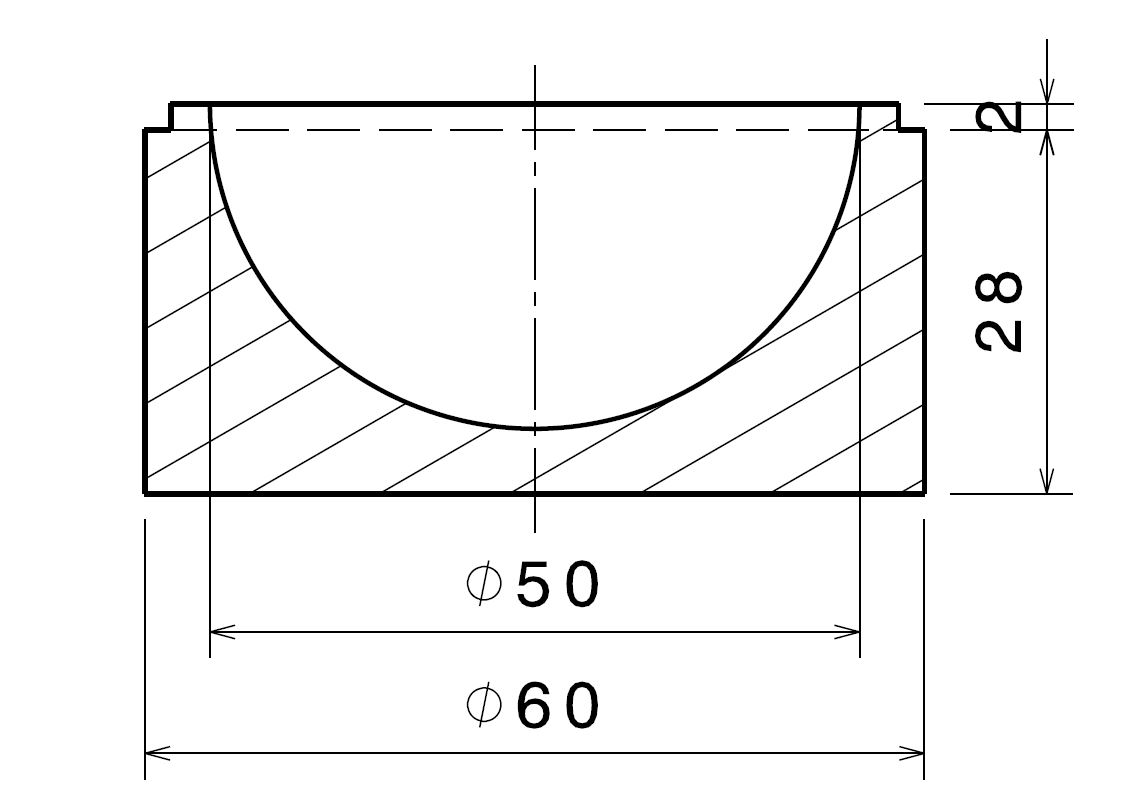
\includegraphics[width=0.48\textwidth]{figures/Chapter_1/female_mold.jpg}%
		\caption{Longitudinal section of the female mold}%
		\label{fig:female_mold}%
\end{figure}


\paragraph{\textbf{Translation guide sleeve:}}
It is a hollow cylinder with an inner radius $R_{in} = R_{cylinder} = 30 mm$, and a thickness of $5 mm$. where the female mold is slid in. It is slightly higher than the female mold by $5 mm$. One extremity is provided with an inner chamfer of $5°$ which ensures the concentricity between the female mold and the male mold.
\begin{figure}[h] %
	\centering%
  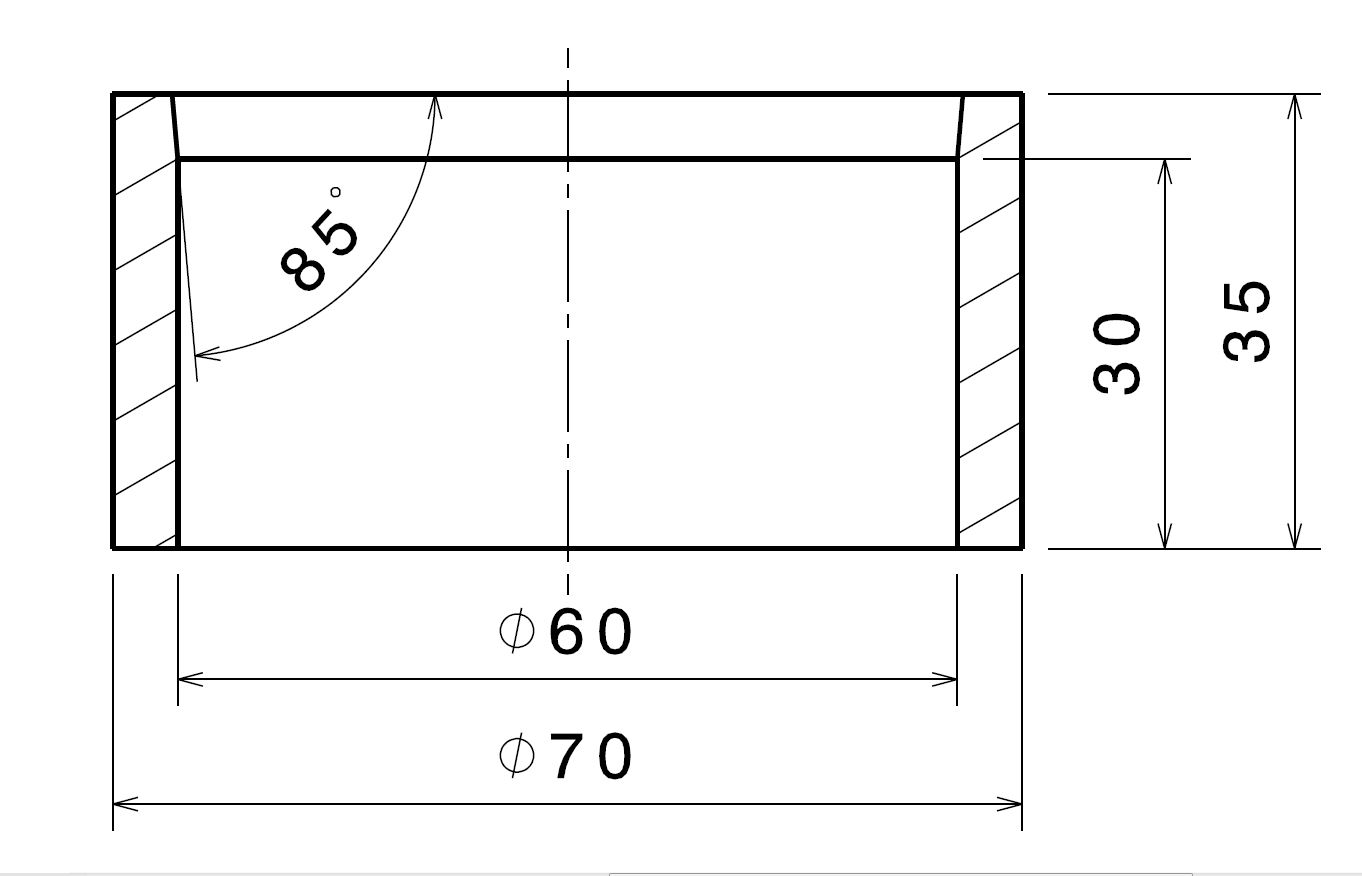
\includegraphics[width=0.48\textwidth]{figures/Chapter_1/sleeve_translation.jpg}
  \caption{longitudinal section of the sleeve}%
		\label{fig:sleeve_1}%
\end{figure}

\paragraph{\textbf{Male mold:}}
Figure \ref{fig:male_mold} shows the design of the male mold which consists of half a sphere of radius $R_{int}<R_{out}$, which is changed to cast different thicknesses. It is supplied with a shouldering which acts as a travel stop, its flanks have a slight angle of 5 providing a translation guide and preventing an over-center locking in combination with the guiding sleeve previously presented. The cylindrical part over the shouldering helps manipulating the mold during the casting process. Three radii have been used: $R_{int} = 18.5 mm, 20 mm, 23 mm$. 
\footnote{All the molding parts presented are made of Aluminum "`Fortal"'. The female and male molds were machined using a CNC (computerized numerical control)  machine and with a precision of $tol =\pm 0.01 mm$. The surface roughness obtained was of $R_a = 0.04$ which indicates a very good finishing.
This choice of manufacturing was unavoidable since no other alternative could produce spherical shapes with such precision conditions.}
\begin{figure}[h] %
	\centering%
  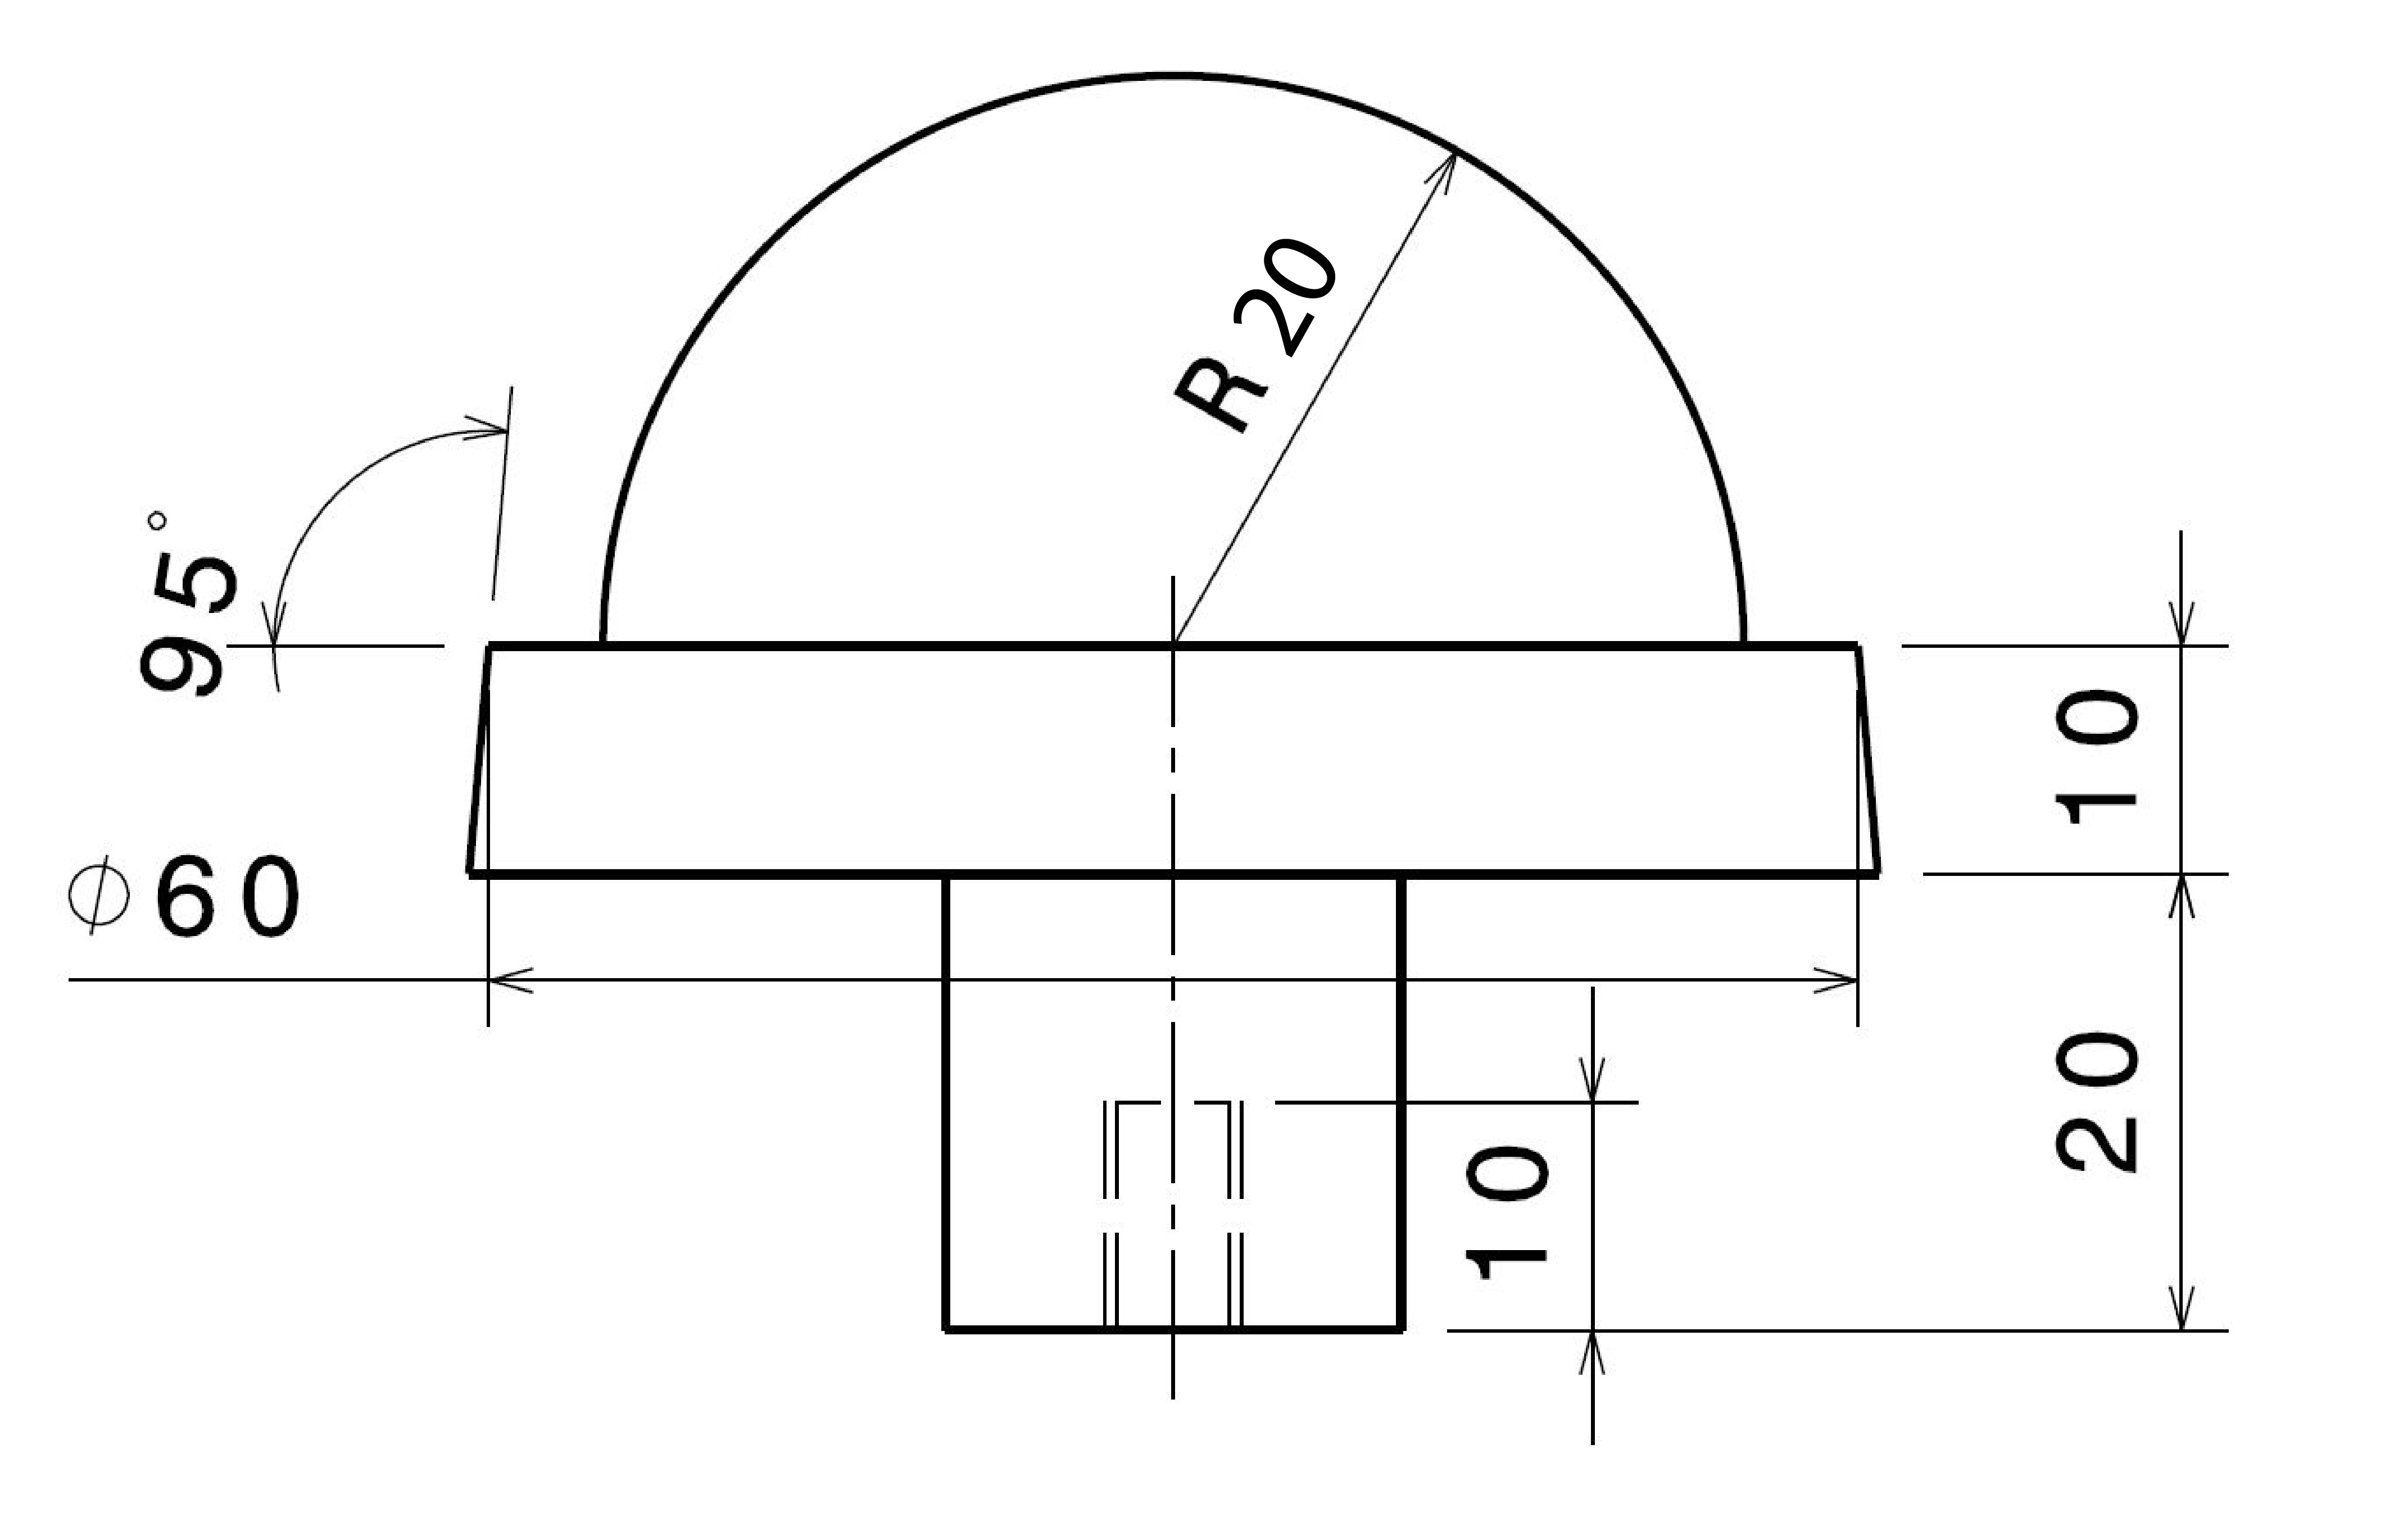
\includegraphics[width=0.48\textwidth]{figures/Chapter_1/male_mold.jpg}
	\caption{longitudinal section of the male mold}
	\label{fig:male_mold}
\end{figure}

\paragraph{\textbf{Gluing sleeve}}
It is a hollow cylinder with an inner radius $R_{in} = R_{cylinder} = 30 mm$, a thickness of $5 mm$ and a height of $50 mm$. It is used during the gluing process to ensure the concentricity of the two halves of the sphere contained in the female molds which face each other.

\paragraph{\textbf{Mechanical press}}
It's a simple press consisting of two metallic plates supplied with a set of threaded rods and hexagonal nuts used to apply pressure over female/male molds during the casting step to prevent bubbles from appearing during the casting step. It is also used during the gluing step on the female/female molds to ensure the contact between the two half spheres to be glued together.

\paragraph{\textbf{Pasta machine}}
This machine (fig\ref{fig:pasta_maker}) consists on two rotating cylinders, with an adjustable inter-space which allows to produce layers with the desired thickness.
\begin{figure}[h] %
	\centering%
  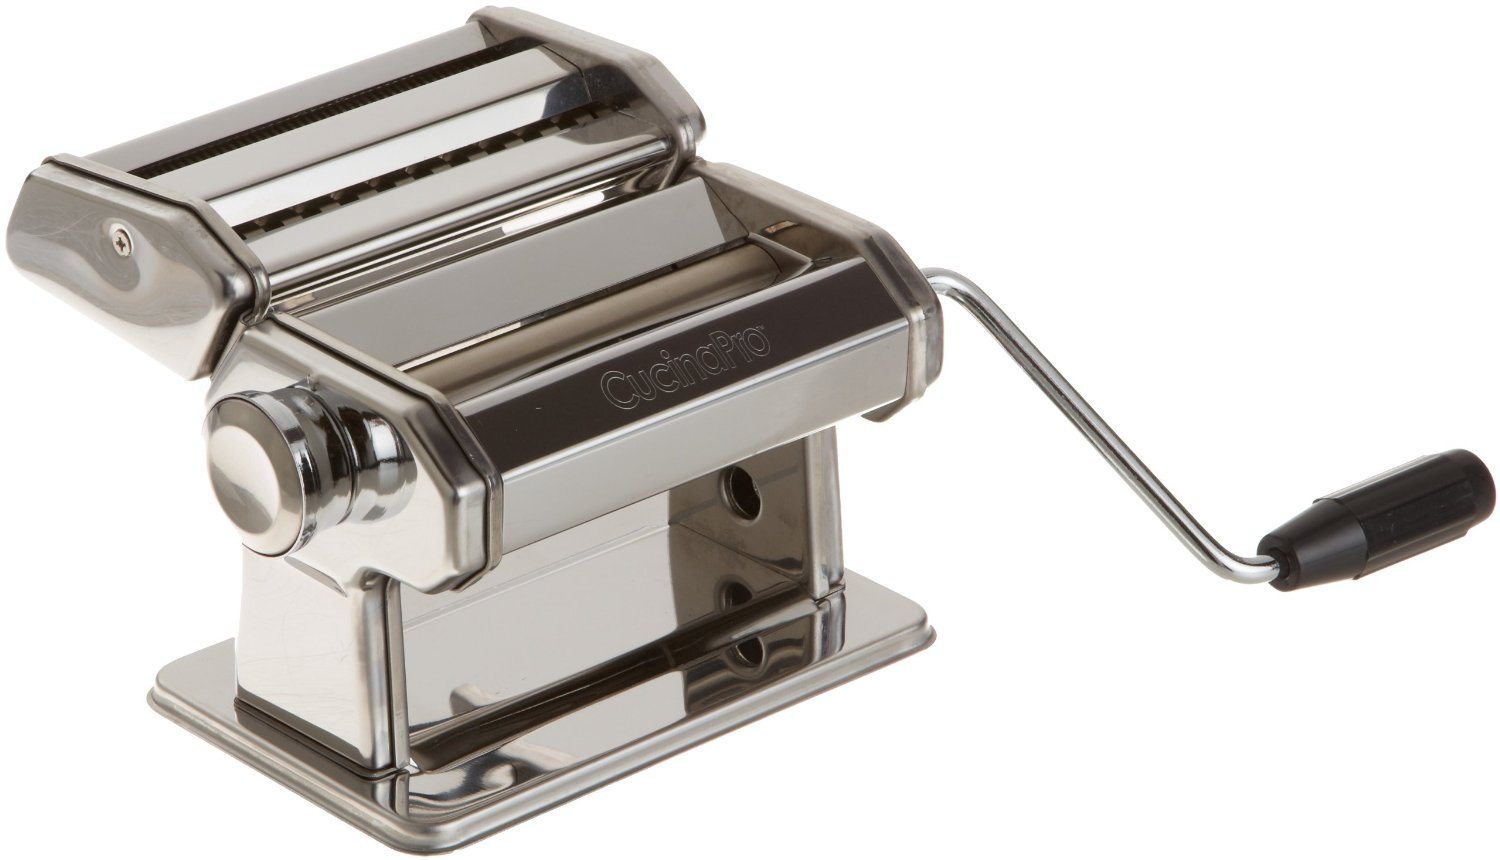
\includegraphics[width=0.48\textwidth]{figures/Chapter_1/rolling_machine.png}
	\caption{Pasta maker}
	\label{fig:pasta_maker}
\end{figure}

\newpage
\subsection{Materials and protocols}
Three materials were used in the experiments done during the study: "`Dragon Skin\textregistered 30"' which has a specific molding protocol and AJO 121 and AJO 122 which have a common molding protocol.

\subsubsection{Dragon skin\textregistered 30} 
\paragraph{}
This material is typically used to make special effects.In the case of our study, it was used to investigate the effect of the $\frac{d}{R}$ on the swimming mechanism. Its exact chemical constitution is not known, but what can be said is that it is cure liquid silicone compound, which consists of two liquid components named A and B. Component \emph{A} represents the silicon polymer chains with eventually the presence of fillers to enhance its mechanical properties. Component \emph{B} is the cross-linking agent providing bonds that link one polymer chain to another, decreasing the flexibility of the polymer chain and increasing its rigidity. Mixing these two components at room temperature, it creates a solid that takes the shape of the container it was poured in.
The typical mechanical properties of the resulting rubber are:
\begin{itemize}
	\item Shore A Hardness : 30 
	\item Specific gravity : 1.08 
	\item 100\% elastic modulus : 0.6 MPa
	\item Elongation at break : 364\%
	\item cure time (at room temperature) : 16 hours
\end{itemize}

\paragraph{Half shell casting}
\begin{enumerate}
	\item Begin by determining the mass of a shell with a outer radius of $R_{out}= 50 mm$ and a thickness $th$ which gives an internal radius $R_{int} = R_{out}-th$, The mass\footnote{In practice, this mass is increased by 50\% to take into account the eventual loss during the preparation.} of a hollow sphere is given by the following formula:
		\[Mass_{shell} = \frac{4\pi}{3}\rho_{material} (R_{out}^3-R_{int}^3) \]

	\item In a beaker, we weigh 50\% of the shell mass of component A which is the silicon polymer chain. We stir thoroughly and add 50\% of the shell mass of component B, which constitutes the cross-linking agent, we stir thoroughly.
	\item The mixture is then degassed thanks to a vacuum pump.
	\item The female and male are cleaned using acetone and 50\% of the degassed mixture is poured in the two female molds.
	\item We degas again to make sure no air was entrapped during the previous step.
	\item Each female mold is slid in the translation guide sleeve and the male mold corresponding to the desired $R_{int}$ is gently slid inside the female mold to prevent air from getting trapped.
	\item The female-male molds assembly is then pressed and locked using the press.\footnote{This step is necessary to ensure that no bubbles get trapped during the assembly.}
	\item The press is then put into an oven at 65°C to speed up the cross-linking process reducing it from 16 hours to only 20 minutes.
	
\end{enumerate}

\paragraph{Half spheres gluing}
Once the two halves of a hollow sphere of the desired $R_{int}$ are cast. We need to glue the two halves together to obtain a complete hollow sphere of thickness $th$.
This part is critical: if the sewing is weak, it will tear apart during the buckling phase. if the sewing is thick, it means that the shape is no longer spherical. If the gluing material is not the same, we lose the homogeneity of the material and potentially create a weak zone at the sewing, which would accelerate the weakening of this zone and ultimately tear apart.
\paragraph{} 
To efficiently glue the two halves and avoid the problems stated previously. We used the same material to perform the gluing, but for that it was necessary to decrease the viscosity of the mixture and enhance its wetting properties. For this purpose, we mixed "`Pentane"' which is an organic solvent \cite{NgLee2003} with a solubility parameter similar to that of PDMS.
The following describes the protocol of gluing:
\begin{enumerate}
	\item Prepare 10g of a mixture A+B of the Dragon skin\textregistered 30 and degas it.
	\item Add 5 ml of "`Pentane"' to the mixture and stir to obtain a diluted mixture that is neither too liquid nor too viscous and pump the resulting liquid inside a syringe.
	\item Use an abrasive such as sandpaper over the gluing area of the two halves casts to make the surface rougher.
	\item Put back each cast in the female mold and align it correctly so that the gluing area is horizontal.
	\item Pour uniformly a layer of the diluted mixture using the syringe needle on the gluing area of both casts.
	\item Put one female mold inside the gluing sleeve, facing upward then slide the second one facing downward until the two gluing areas are in contact.
	\item Ensure the contact by using the mechanical press and let the cross-linking happen at room temperature for 16 hours.\footnote{This time we don't use the oven to ensure that the pressure inside the spherical hollow shell is the atmospheric pressure.}
	\item After the curing time, remove the residual thin skin circling around the sewing area.
\end{enumerate}
  

\subsubsection{AJO121/122}
\paragraph{}
The two remaining materials \emph{AJO 121} and \emph{AJO 122} were samples kindly supplied by "`\textbf{BLUESTAR silicones\textcopyright}"'.Both are hot curing silicone rubbers after addition of a vulcanization agent. The typical applications of these materials are: molding and injection molding process for technical parts (sealing gaskets,grommets), extrusion profiles (windows profiles, sleeves, tubes) and calendering operations for manufactured hoses. They were chosen to investigate the effect of solid dissipation characterized by the rebound resilience property. This pair of materials present the particularity of sharing the same elastic energy storage capacity characterized by the elastic modulus.In the case of the samples provided by "`\textbf{BLUESTAR silicones\textcopyright}"', both material present a soft white paste-like texture. The exact chemical composition of the pastes were not disclosed but what we know is that the curing agent, which is 1.25 \% of \textbf{2,4-dichlorobenzoyl peroxide}, was already mixed with the silicone polymer. The vulcanization process is temperature-controlled and is induced at 115°C.\\

The typical mechanical properties of the resulting rubbers are:
\begin{itemize}
	\item 100\% elastic modulus AJO121 / AJO122 : 2.2 MPa / 2.3 MPa
	\item Rebound resilience AJO121 / AJO122 : 45\% / 65\%
	\item Shore A AJO121 / AJO122 : 60 / 59 
	\item Specific gravity : 1.16
	\item Elongation at break AJO121 / AJO122 : 560\% / 366\%
	\item cure time (at 115°C) : 10 minutes
\end{itemize}

\paragraph{Half shell casting}
\begin{enumerate}
	\item Begin by determining the mass of a shell with a outer radius of $R_{out}= 50 mm$ and a thickness $th$ which gives an internal radius $R_{int} = R_{out}-th$, The mass of a hollow sphere is given by the following formula:
		\[Mass_{shell} = \frac{4\pi}{3}\rho_{material} (R_{out}^3-R_{int}^3) \]

	\item Weight the calculated mass from the paste and divide it in two equal parts.
	\item Press each part at the center of the female mold.
	\item Each female mold is slid in the translation guide sleeve and the male mold corresponding to the desired $R_{int}$ is slid inside the female mold.
	\item The female-male molds assembly is then pressed and locked using the press.
	\item The press is then put into an oven at 115°C to trigger the vulcanization process, during 8 minutes \footnote{This period was reduced to 8 minutes instead of 10 minutes to avoid reaching the maximum of the cross-linking, in order to complete the gluing}.
	\item A post-curing at 200°C is needed to optimize the mechanical properties of the material, to evaporate remaining volatile substances (sub-products linked to the peroxide) and allow the sublimation of the 2,4 Dichlorobenzoic acid which manifests as a white powder at the surface of the material, at the end of the previous step.
\end{enumerate}

\paragraph{Half spheres gluing}
The gluing using the AJO materials was very challenging for different reasons. First, the paste-like nature of the material which was not soluble in any organic solvent without compromising the vulcanization agent already mixed with the raw polymer. It also made manipulating it harder, contrary to the liquid nature of the "`Dragon Skin\textregistered 30"'. Second, we were not able to glue together two flat surfaces, due to the fact that the cross-linking process reached a maximum with the prescribed time and temperature and no biding was possible afterward.
This is the protocol followed which solved partially the problems previously stated:

\begin{enumerate}
	\item Prepare two thin layers (0.1 mm) using the "`pasta maker"' machine. Adjust their width to 10 mm and the length to $2\pi R_{out} \approx 157 mm$.
	\item Use an abrasive such as sandpaper over the gluing area of the two halves casts to make the surface rougher.
	\item Put back one cast in the female mold and align it correctly so that the gluing area is horizontal.
	\item Put uniformly a first layer on the gluing area of one cast and make sure it adhered to the surface, cut the residual width using a scalpel.
	\item Connect the remaining half (without the female mold) with the first and press to get and adhesion.
	\item Put one female mold inside the gluing sleeve, facing upward then slide the second one facing downward until the two gluing areas are in contact.
	\item Remove the female mold gently and roll the second layer around the sewing perimeter, taking care not to disconnect the two halves while doing so.
	\item Encapsulate the shell inside the two female molds and exert pressure using the mechanical press.
	\item Put the press inside the oven at 115°C for 10 minutes. Remove it and let it cool at room temperature.\footnote{The capsules produced using this protocol have an internal pressure close to $75\%$ of the atmospheric pressure.}
\end{enumerate}
